\chapter{High-Level Architecture}
% this architecture was motiviated by design decisions, here is the list of decisions 1 2 3 4, now let us work each one of those design decisions out in detail in the following sections.

Calico's new architecture was motivated by the design decisions listed below. The key design decisions for the new version of Calico were:

\begin{itemize}\itemsep1pt
  \item Client/Server architecture for improved connectivity over the internet.
  \item Optimization of network traffic to reduce lag on distant clients, as well as network usage.
  \item A plugin framework to easily enable developers to create extensions into the Calico system.
  \item Improvement of input event handling system to improve drawing performance and input recognition.
  \item Consistency handling and persistence improvements to ensure that clients are all kept in the same state.
\end{itemize}

In the following sections, each decision will be explained in more detail.



\section{Client/Server Architecture}
In order to meet the objectives that we set in the new version of Calico, we decided that the architecture needed to be redesigned in order to support all the changes. The new architecture that was chosen had to be able to support all the features, as well as easily support multiple users simultaneously. It also had to be accessible from anywhere, and had to be more stable than previous versions that were known to crash.

\begin{figure}[h]
\centering
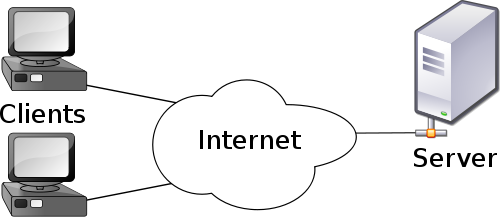
\includegraphics[width=0.8\textwidth]{fake_arch.png}
\caption{Overview of Calico's Architecture}
\label{fig:calico_arch}
\end{figure}

The first change made was a switch from the original peer-to-peer system to a completely new client-server architecture. We believed that by using the client-server architecture, we could provide a centrally accessible service that would easily support multiple clients and still maintain stability. The server could act as a headless service that could be very powerful since it did not have to perform any client functions. This meant that the server could be dedicated to the task of managing all the interactions between clients, and could be much more stable than in a peer-to-peer context.
\todo{Not deep enough, *) simple *) single point of failure}

\section{Networking Component Overhaul}
One of the significant changes from the original Calico was the change in network communication design. The previous version of Calico had networking that was designed as a plugin, and was not fully integrated into the system. In this old design, when a change was made by another client, the entire change was saved to a Java object. This object was then serialized and sent in full over the network. The receiving client would deserialize this data, and then perform the change on its local drawing canvas. This process was very easy to implement, but had the cost of processor time due to the constant serialization/deserialization process that would take place for each action. It also incurred the network overhead of Java serialization, which would add much more data to the final packet then would ever be needed. All of this overhead would quickly become apparent to users when the system would lag in response to many actions done in quick succession. Our goal was to streamline this process as much as possible so that we could reduce lag when the system was being heavily utilized.

To improve the responsiveness of Calico, and reduce the network overhead, we created a custom packet design that could be used by Calico to notify both the client and server when various actions were performed. These special packets provided exactly what was needed to effectively communicate changes to clients, and were reduced to the minimum size. Packets were byte arrays that were written directly to the wire, and based on various settings, they could be decoded back into their specific components. 



\begin{figure}[h!]
  \centering
  \begin{bytefield}{34}
    \bitbox{4}{length} & \bitbox{8}{command ID} & \bitbox{24}{command-specific data}
  \end{bytefield}
  \caption{A Calico network packet}
\label{fig:calico_packet}
\end{figure}

This packet design was loosely based on the packet design of the Half-Life game engine \cite{rcon}.As seen in the figure above, the packet was broken up into three main parts. The first four bytes of the packet was the length of the packet. This would tell the network system how much farther it needed to read to ensure it received the entire packet. The next four bytes held the command identifier. This number was used to tell the network system what this packet was about. Both the client and the server had a list of commands and their IDs, which was used to translate from a programmer-friendly command name to the command ID number. The remaining bytes could vary based on the specific command that was given. Each command had different parameters, which both the client and server were aware of, and could decode the packet into specific commands. By writing data directly to the wire, there was no overhead at all with inflated packet sizes -- each packet was as small as it could be. This made the network communication between the client and server more efficient, and helped to reduce the lag, even when put under heavy usage.
% PD: How did you test this?

\section{Plugin Framework}
To improve the extensibility of Calico, a plugin framework was created. This plugin framework allowed for extra features to be easily integrated into Calico. Plugins could subscribe to specific events that they wanted to be notified about. When one of these events was triggered within Calico, all subscribers to that event were notified, and could perform any action based upon the event information. 

To create a plugin, developers only had to extend a provided abstract plugin class that allowed each plugin to register itself with a \texttt{PluginManager} that was responsible for publishing network events and interface events to each plugin. Plugins were provided with default ``hooks'' that would be called upon when the plugin was loaded or unloaded. Plugins were able to call a method \texttt{registerNetworkCommandEvents} that would allow it to subscribe to specific network commands that it was interested in. Another method, \texttt{RegisterPluginEvent} enabled the plugin to subscribe to various interface events that could be used for processing user input and clicks. This plugin system provided a very easy way for developers to interact with the Calico framework, without needing to modify the code of the existing system. Developers could quickly create plugins that could interact with a live system.


% \todo{ANDRE: Proof comes later in thesis}
% In the early stages of new Calico, the plugin framework was used to recreate the palette feature that existed in the original Calico.
% DesignMinders\cite{todo}, a system that <DOES SOMETHING> was also able to interact with Calico using the plugin framework. Designers could take a snapshot of their current design, and this snapshot would be recorded and annotated by the DesignMinders system. The interaction with DesignMinders was positive proof that the plugin framework offered exceptional power to developers who wanted to interact with Calico.

\section{Improvement of Input Handling System}
In the previous version of Calico, the input system was plagued by sluggish performance and inaccuracy. When there were many elements on the screen, the input system would lag and would begin to ``miss'' input data, which would result in straight lines instead of smooth curves. As a sketching tool, the ability to receive accurate input from the user was very important to the performance of the tool. The previous version of Calico routed input data directly to the rendering system which would draw the images on screen. This made development very easy, but it required the input system to wait on the rendering process. This meant that the more images that had to be rendered, the longer the input system had to wait before it could start processing new input data. In Java, the mouse input listener does not queue input events --- if a program is too busy to receive input, then that input event is lost forever. Due to this problem, fluid drawing was nearly impossible.   

\todo{ANDRE:Add an architecture diagram?}
The new version of Calico was designed to fix this problem. By creating a separate, but dedicated input handling system, Calico could readily receive input commands without having to wait for rendering process to complete.
\todo{Give more examples}
Instead of linking the input, action processing, and rendering systems serially, they were linked in ``parallel'' using a multi-threaded approach. None of the separate processes were reliant on any of the other processes to complete, and so input could be quickly received and queued if needed. These input events were then sent to the action processing system which determined what actions if any should be performed based upon the given input. Once an action was decided, the rendering process was notified and could then redraw the screen as needed. By using these systems in parallel, we were able to remove the perceived lag and missed mouse events that would cause distortion and incorrect sketching. By capturing input events and queuing them, we were able to capture more detailed input, which allowed the board to continue capturing events while the interface was rendering the display. This meant that while the display could lag slightly behind the rendering system, the delay was not nearly as noticable as when input events were being missed. 

% Maybe talk about mouse location problems? 
% Problems tracking where the mouse was

\section{Consistency Handling / Persistence}
The previous version of Calico had many problems maintaining consistency between all clients. Clients would quickly become outdated and their states would not be consistent with that of the other clients. 
This problem was generally a result of parallel edits being performed. Clients would perform the edits locally, and then notify the other clients of the change. Often, the events would be received in a different order than they were being performed on a client, and the elements would be modified incorrectly. This led to identical elements being displayed very differently on multiple clients, due to the fact that there was no authoritative server to solve disputes when edits were being done to an element at the same time.
The previous version of Calico had no central server to check or update consistency, so any time where a client became inconsistent, designers had to quit the program and reconnect in order to fix the problem.
Naturally, this was very frustrating to users as it made it very difficult to collaborate with another user once the data became inconsistent. 

In the new version of Calico, this problem was fixed by implementing a system for checking and maintaining consistency across all clients connected to the server. In the new Calico, the server was considered to be the master, and all clients would defer to the server to determine what state they should be at. All client actions were sent to the server and were not processed on the client until the server acknowledged the command. This meant that all clients were given the same commands to modify elements at the same time. Clients were essentially ``unintelligent'' and did not assume any knowledge of where elements should be positioned --- this was all maintained by the server. This meant that clients never became inconsistent, as there was a single system that was responsibile for maintaining the state on each client system. 
Even when clients were editing the same element in parallel, Calico was able to maintain consistency by giving priority to the first event received. This would allow users to edit the same element, and prevented the system from trying to issue conflicting edits to the same object.
The only time when clients would lose consistency was during network errors where packet loss was experienced. However, even if this were to occur, there were regular consistency checks that would quickly realize the inconsistencies and fix them, without ever interrupting the designer.
\todo{Give example, talk about user's perspective}

To account for situations where packet loss was inevitable, a consistency management system was created that would periodically notify all clients of the current state of the system. The consistency check was performed by sending a hash code to all clients that represented a checksum of the system and all the components. If any of the clients responded with a different hash code, they were sent an export of the entire session which contained all the data needed to essentially recreate the session from scratch. Because of this, any inconsistencies could easily be mitigated with minimal inconvenience to the end user. This meant that a session using the new version of Calico could last for weeks without problem --- something that was not possible in the previous version of Calico.
% How data is sent back and forth between server and client
% How data is written to the controllers
% how parallel edits are dealt with




%%%%%%%%%%%%%%%%%%%%%%%%%%%%%%%%%%%%%%%%%%%%%%%%%%%%%%%%%%%%%%%%%%%%%%%%%%%%%%%%%%%%%%%%%%


%\section{Major Changes}
% move away from java objects being sent over the wire
% describe packet system

%\section{Maintaining Consistency}
% How data is sent back and forth between server and client
% How data is written to the controllers
% how parallel edits are dealt with
% 

%\section{Server Architecture}


%\section{Client Architecture}

% Components
% - Server
% - Client




% ANDRE NOTES

% we were motivated in this and this way
% we build arch shown in figure 2
% the key design decisions are
%      - this one
%      - this one
%      - this one
% let us talk about each one of those design decions in detail in each of the sub sections


% page or two that is a general intro to the higher level arch


% new arch is client/server, new arch uses specialized messages, the internals of the server have X components, the internals of the client have Y components


% take out problem stuff, put in diff sec
% this section = your arch and your key design decisons


% this architecture was motiviated by design decisions, here is the list of decisions 1 2 3 4, now let us work each one of those design decisions out in detail in the following sections.
% (take each design decision and take time to explain it) list out all important design decisions


% Client Server Arch
% several alternatives were considered
% -- we could have updated the P2P architecture, we could have done a standalone system, we could have done a bus system, but for the reasons of consistency, persistence, control, extensibility, we decided to make client/server. Explain some alternatives, and why we didnt pick those


% - Client Server Arch
% - Optimize network traffic
% - extension points (plugin framework)
% - event handling (input interface)
% - consistency handling / persistence
